%%%%%%%%%%%%%%%%%%%%%%%%%
% Set up to be stand alone document
% All declerations in the header to be removed when added into thesis
%%%%%%%%%%%%%%%%%%%%%%%%%
% \documentclass[12pt]{article}

% \usepackage{booktabs} % booktabs provides professional formatting commands for tables
% \usepackage{amsmath} % amsmath provides extra maths symbols
% \usepackage{textcomp} % textcomp provides extra text symbols (like a degrees celsius symbol)
% \usepackage{../customisations}
% \usepackage{natbib}

% \title{$J$-band Sythentic Spectral Fitting}
% \date{\today}

% \begin{document}
% \maketitle
%%%%%%%%%%%%%%%%%%%%%%%%%
% To be included when added into thesis
\chapter{J-band Sythentic Spectral Fitting}
\label{ch:janal}

\section{Opening Remarks} % (fold)
\label{sec:opening}

In this chapter I describe in detail the process by which I implement an analysis
routine to fit synthetic spectra to observed data with the aim of estimating stellar parameters.
This analysis builds on existing methods while providing a fresh approach to various aspects of the routine.
I have developed this implementation in the public domain and the source code for this project is made publicly available
via an online repository.\footnotemark

\footnotetext{Souce code available from: https://github.com/lrpatrick/rsg-janal
although the interested reader should be aware that these routines are, at the time of writing, in development mode
in the sense that they are highly specialised to one machine and (particularly) one set of model grids}

In this chapter I first outline the principles of model atmospheres~\ref{sub:model_atmospheres}.
Where I discus the physics which is included in these models, some of their strengths and their limitations.
I then focus the discussion on the grid of synthetic stellar spectra which forms the base of this analysis routine in~\ref{sub:model_grid}.
In~\ref{sub:continuum_fitting} I detail the procedure of matching the continuum level of the observations with that of the models,
which leads on to~\ref{sub:best_fit_parameters} where the method by which the best fit parameters are selected is described.

Having described the analysis routine thoroughly I then test this routine and compare the results of this method to different implementations in~\ref{sub:compare}.
Finally, I conclude the chapter in~\ref{sub:conclusions}.

% section opening (end)
\section{Introduction to Stellar Model Atmospheres} % (fold)
\label{sub:model_atmospheres}

A stellar atmosphere is defined as the outer layers within a star which emitt radiation.
Therefore, by definition, the photons which we observe from a star have originated in the atmosphere.
Photons which have originated from deeper layers within the star have been absorbed and re-emitted by particles within the stellar atmosphere.
Stellar atmospheres are therefore vitally important in observational studies of stars, even though the fraction of the total mass of the star contained within the atmosphere is tiny ($\sim$~10$^{-10}$).
A nice analogy for visualising this layer and its thickness comes from the preface of~\cite{1989isa2.book.....B}, where these authors compared the skin of an apple to a hypothetical star which has been shrunk to the same scale and note that the skin of the apple is far thicker than the stellar atmosphere.


Even though stellar atmospheres contain a tiny fraction of the total stellar mass, these layers can have an enormous impact on the evolution of a star via stellar winds.
For example, in evolved massive stars, winds arising from the atmosphere can strip off the outer layers of the star to leave an exposed hydrogen and helium dominated core or push the star in a completed different evolutionary direction to become a RSG (see Chapter~\ref{ch:intro}).
In addition to having an impact on the evolution of the star, winds also help distribute material throughout their host galaxy and feed subsequent generations of star formation~\citep[e.g.][]{2011MNRAS.417..950H,2012MNRAS.421.3522H} thereby not only affecting the evolution of the star which the wind is produced, but by acting as part of a larger stellar population, affecting the evolution of their host galaxy.

By modelling stellar atmospheres, one can estimate fundamental stellar parameters by a comparison with observations.
The background theory and underlying physical assumptions of these models is the subject of the current section.
This is important to detail as without this background it is impossible to asses the effectiveness of the models and their limitations.

Two of the most fundamental equations which govern the properties of stellar atmospheres are,

\begin{equation}
    g = \frac{GM}{R^2},\label{eq:grav}
\end{equation}

\noindent and,

\begin{equation}
    T_{\rm eff} = \frac{F}{\sigma_{SB}} = \left(\frac{L}{4\pi \sigma_{SB}R^2}\right)^\frac{1}{4},\label{eq:Teff}
\end{equation}

\noindent where $g$ is the acceleration due to gravity, $M$ is the total mass of the star of radius $R$, $T_{\rm eff}$ is the effective temperature of the star, $F$ is the total flux per unit area, $L$ is the total luminosity of the star, $\sigma_{SB}$ is the Stefan-Boltzmann constant,  and $G$ is Newton's gravitational constant.

These equations define some fundamental observational properties of the model stellar atmospheres, using fundamental parameters of the models.
Equation~\ref{eq:grav} is defined by the density stratification of the model and equation~\ref{eq:Teff} is defined through the total flux emitted from the model.

In the following sections I detail three of the principle assumptions which are used to create a ``classical'' one dimensional stellar model atmosphere.
These assumptions underpin some of the most widely used model atmospheres.


\subsection{Hydrostatic Equilibrium} % (fold)
\label{sub:hydrostatic_equilibrium}

Any model of a star consists of a balance bewteen gravity and pressure in a gaseous material (or plasma considering the typical temperatures and densities within a star).
If a model is assumed to be static (i.e. not varying with time) the equation of hydrostatic equilibrium can be derived by considering the balance between the forces acting upon a small element of stellar material,

\begin{equation}
    \frac{dP(r)}{dr} = -\frac{\rho GM(r)}{r^2},\label{eq:hydro}
\end{equation}

\noindent where $P$ is the total pressure exerted within a radius $r$, $M$ is the total mass within a radius $r$, $\rho$ is the matter density~\citep[see Chapter 9 of ][for a simple derivation of this equation]{1989isa2.book.....B}.
As stated above, the mass contained within the atmosphere of a star is a negliable fraction of the total mass, therefore $M(r) = M_{tot}$ when considering this equation in the outer layers of the star.

The force exerted by pressure acting on an element of stellar material ($dP/dr$) can be considered as the sum of the forces acting upon it from gas pressure ($P_{g}$), radiation pressure ($P_{rad}$) and turbulent pressure ($P_{turb}$),

\begin{equation}
    \frac{dP_{tot}}{dr} = \frac{dP_{g}}{dr} + \frac{dP_{rad}}{dr} + \frac{dP_{turb}}{dr}.\label{eq:pressure}
\end{equation}

Equation~\ref{eq:pressure} illustrates that even though we have assumed the model is static, small scale turbulent motions must still be taken into account to accurately model stellar atmospheres.


% subsection hydrostatic_equilibrium (end)

\subsection{Mixing Length Convection} % (fold)
\label{sub:mlt}

Mixing length theory describes how convection is treated within the stellar atmosphere.
Typically, within a star, radiation is the main source of energy transport as the coefficient of diffusion is far smaller for particles (conduction) than for photons (radiation).
Only in degenerate cores does energy transport via conduction become important.

Convection is a very efficient form of energy transport where a macroscopic element of higher temperature rises an average distance into a region of lower temperature where it dissipates the excess energy being carried and mixes.
However, in order for convection to be effective, a driving mechanism must be established.
The atmosphere is unstable to convection if the Schwarzschild certerion is met,

\begin{equation}
    \nabla_{rad} > \nabla_{ad}
\end{equation}

\noindent where $\nabla_{rad} = (d~{\rm ln}\,T/d~{\rm ln}\,P)_{rad}$ is the radiative temperature gradient and $\nabla_{ad}$ is the adiabatic temperature gradient.
The driving mechamism for convection is usually a large temperature gradient within a particularly part of the star.
This can occur at various stages within the lifetime of a star, for example, most main sequence stars have a convective core which is a result of the temperature sensitivity of the CNO cycle which establishes a steep temperature profile.

The theory of convection is very difficult to to treat thoroughly.
The ``simple'' theory of mixing length convection~\cite{1958ZA.....46..108B,1965ApJ...142..841H} is widely used to implement convection within stellar atmospheres which assumes that the shapes and sizes of the elements which transport energy is fixed and that, on average, an element rises a characteristic length ($l_m$) before it dissipates energy.

If the Schwarzschild criterio is satisfied, the total flux ($F$) for a star is given by,

\begin{equation}
    F(r) = F_{conv} + F_{rad} = \sigma T_{eff}^4,\label{eq:flux}
\end{equation}

\noindent where $F_{conv}$ and $F_{rad}$ are the convective and radiative flux respectively.
An expression for the convective flux can be obtained by considering the excess energy dissipated by a rising element moving a distance
($\Delta r = l_m/2$) with an average velocity ($v_{conv}$).
The convective flux can therefore be expressed as,

\begin{equation}
    F_{conv} = \rho C_pv_{conv}\Delta T
\end{equation}

\noindent where $C_p$ is the specific heat at constant pressure and $\Delta T$ is the temperature difference between the element and surroundings, which can be expressed in terms of the different in temperature gradients.
Here the pressure scale height can be introduced using the assumption of hydrostatic equilibrium $H_p = dr / d{\rm ln} P = p/\rho g$ and an expression for the convective velocity can be estimated by assuming that half the work done by bouyancy is converted into kinetic energy,

\begin{equation}
    \frac{1}{2}\langle w\rangle \approx \frac{1}{2}\rho v_{conv}^2.
\end{equation}

The parameter $\alpha = l_m/H_p$ is introduced which typically takes the value $\alpha = 1.5--2.0$.
As a side note, in stellar evolutionary models, the value of $\alpha$ used can have a significant effect on the temperature of the models at the end of the RSG phase of evolution.


% subsection mlt (end)

\subsection{Local Thermodynamic Equilibrium} % (fold)
\label{sub:local_thermodynamic_equilibrium}

The assumption of thermodynamic equilibrium is where the temperature and density of a material can be considered constant (i.e. there are no net flows of energy).
Which is equivalent to assuming that the emitting source is a perfect black body.
Local thermodynamic equilibrium (LTE) is an approximation whereby the {\it local} properties of material can be assumed to be in thermodynamic equilibrium.
Stellar atmospheres can be approxmiated to be in LTE as their densities are sufficiently high that and density gradients are sufficiently low that their local properties are closely related to thermal equilibrium.

The three fundamental equations which can be defined assuming LTE are:

\begin{enumerate}
    \item The Boltzmann equation,
    \begin{equation}
        \frac{n_i}{N_I} = \frac{g_i}{U_I}e^{-E_i/kT},
    \end{equation}
    \item The Saha equation,
    \begin{equation}
        \frac{N_I}{N_{I+1}} = n_e\frac{U_I}{U_{I+1}}\left(\frac{h^2}{2\pi m_ekT}\right)^\frac{3}{2} e^{\chi/kT},
    \end{equation}
    \item The Maxwellian distribution of particles,
    \begin{equation}
        f(v)dv = \left(\frac{m}{2\pi kT}\right)^\frac{3}{2} \exp\left(\frac{-mv^2}{2kT}\right)4\pi v^2dv,
    \end{equation}
\end{enumerate}

\noindent where $n_i$, $g_i$ and $E_i$ are the population, statistical weight and energy of level $i$ respectively,
$N_I$, $U_I$ and $\chi_I$ are the total number density, partition function and ionisation potential of ionisation state $I$ (to which $i$ belongs),
$m$ is the mass of the particle, $v$ is the velocity of the particle, $T$ is the temperature of the particle and $k$ is the Boltzmann constant.

% These three equations describe the


% In addition the radiation source function (in the MARCS models -- not always the case) is assumed be be

% \begin{equation}
%     S_\lambda = \frac{\kappa_\lambda}{\kappa_\lambda + \sigma\lambda}B_\lambda(T) + \frac{\sigma_\lambda}{\kappa_\lambda + \sigma\lambda}J_\lambda
% \end{equation}

% More generally, in thermodynamic equilibrium $S_\lambda = B_\lambda$.
% In LTE

% subsection local_thermodynamic_equilibrium (end)

\subsection{Analysis of Assumptions and Summary} % (fold)
\label{sub:assumptions_summary}

The assumptions listed above allow one to obtain to create a ``standard'' stellar model atmosphere.
The assumptions listed above are known to be simplifications of the true picutre witih a stellar atmosphere.
For example, the assumption of LTE definitely breaks down in the atmospheres of stars as they are observed, and by definition emitt radiation.
However, using the above assumptions one can build a consistent model that, in general, agrees reasonably well with observations.

The treatment of convection is knowingly a large simplification as the shape and size assumed for the convective elements is constant whereas in reality the shapes of these elements could be described as funnel-like.
Full two- and three-dimensional hydrodynamical simulations are required to asses the assumption of mixing length convection which generally show that convective fluxes are smaller than those in more sophisticated prescriptions
\citep{2012sse..book.....K}.

The assumption of LTE typically holds in dense low levels of a star, however, in the atmosphere, where radiation is emitted, this is known to be a poor approximation.
This is particularly true in evolved stars where departures from LTE are expected owing to the low densities and surface gravities of their atmospheres.

Full non-LTE stellar model atmospheres are expensive to produce and as of yet, there exists no homogenous grid of model atmospheres which include these effects.
As a first step, one can use a homogeneous set of model grids computed in LTE and select particular elements with which to compute non-LTE deviations.
This is far less time expensive and produces reliable results over a large range of stellar parameters.


% subsection analysis_of_assumptions_and_summary (end)

% section model_atmospheres (end)

\section{Measuring Stellar Parameters with Synthetic Spectra} % (fold)
\label{sub:model_grid}

\begin{itemize}
    \item What are Synthetic Spectra?
    \item Why are they useful?
    \item Background to the J-band method
\end{itemize}

The spectra cover the $J$-band, specifically the $1.16-1.22\mu$m region, where there are various prominent spectral features.
These spectral features, arising from elemental absorption, are compared in the observed and model spectra,
where the $\chi^{2}$-statistic is calculated to asses the goodness of fit for each model.
The stellar parameters which are fit for in this analysis are global metallicity ($log (Z/Z_{\odot})$~=~[Z]), effective temperature (T$_{\rm eff}$), microturblence ($\xi$) and surface gravity ($log\,g$).
% In addition to these parameters, in the future I also hope to further develop this implementation to include the $\alpha$-to-iron ratio as a free parameter.
The observed spectra are fit with models from a set of MARCS model atmospheres
\citep{2008A&A...486..951G}.

The wavelength range, over which to perform this analysis,
is chosen based on the spectral appearance of the region.
Typically, in the spectra of cool stars, dense molecular absorption fetuares dominate the spectrum which require high-resolution spectroscopy to distinguish individual features and estimate stellar parameters in the $J$-band~\citep{Cunha07, Davies09a, Davies09b}.
However, in this small wavelength range the absorption is dominated by well separaeted elemental absorption features from iron, magnesium, silicon and titanium.
Therefore, the spectral resolution required in order to derive stellar paramters is significantly reduced.
This means that this analyis can be preformed with a relatively small amount of telescope time using multi-object spectrographs like the $K$-band multi-object spectrograph (KMOS)
or the multi-object spectrometer for infra-red exploration (MOSFIRE) and is therefore feasible for studies of red supergiant stars (RSGs) in external galaxies.

In addition to this, given the cool temperature of the outer layers of RSGs,
the peak brightness of a typical RSG is $\sim1.1\mu$m.
Combining this with the fact that dust attenuation is significantly lower in the near-IR, compared to the optical regime, RSGs are ideal candidates to be studied at large distances.

Previous implemenations of this analysis include that of
\cite{2010MNRAS.407.1203D} and Gazak (2014).
This implemenation includes aspects of both of these previous implementations and could be described as a hybrid of the two.
Eventually this analysis routine will be made publicly available will should encourage the community to engage with these routines.



The synthetic spectra used in this analysis is based on model atmospheres computed from the
MARCS model atmospheres project~\citep{2008A&A...486..951G}.
These model atmospheres are one-dimensional models (i.e. spherically symmetric)
computed within local thermodynamic equilibrium (LTE).
% where standard mixing-length theory is assumed.
The MARCS models are particularly general and widely applicable to many different types of stars and as such are well used and tested.
However, for the atmospheres of RSGs the assumptions which go into these models are known to break down
\citep{2002AN....323..213F,2010ASPC..425..124P},
therefore, in order to accurately analyse the spectra of RSGs additional corrections must be applied.

The MARCS model atmospheres used for this analysis are computed with a mass of $15M_{\odot}$.
The typical mass range of a RSG is $8~\textendash~40M_{\odot}$, however,
using this mass is applicable owing to the fact that altering the mass of these models affects only the extension
(or geometrical thickness) of the models which does not change for red giants or supergiants
\citep{2010MNRAS.407.1203D}.

To improve the accuracy of the model atmospheres,
non-LTE calculations have been performed for all elements which give rise to the diagnostic features within the wavelength range studied
\citep{2012ApJ...751..156B,2013ApJ...764..115B,2014arXiv1412.6527B}.
% and therefore all of the lines used as diagnostic lines have non-LTE calculations preformed.
Line profiles and non-LTE corrections are calculated using an updated version of the SIU code
\citep{1999PhDT.........3R,2012ApJ...751..156B}.

The parameters of the resulting grid of model spectra are detailed in
Table~\ref{tb:grid}.
The model spectra are at $R~=~10\,000$,
which is chosen to be significantly higher than the typical resolution of the observed spectra
(i.e. $R~\sim~3000$).
The sensitivity of each diagnostic line for a given free parameter is illustrated in figures~\ref{fig:mod-z} through~\ref{fig:mod-micro}.

From an analysis of figures~\ref{fig:mod-z} and~\ref{fig:mod-g} it can be seen that the effect of increasing the metallicity of the models is similar to that of decreasing the surface gravity.
It is therefore expected that a degeneracy exists between metallicity and surface gravity.
This degeneracy is explored further in~\ref{sub:best_fit_parameters}.

The effect of varying the temperature of the models changes the relative strengths of the lines of different spectral species.
For example, see the left panel in Figure~\ref{fig:mod-t} where the ratio of the iron
($\lambda\,1.188285$) to titanium ($\lambda\,1.189289$) lines is strongly affected by varying the temperature of the models.
Also note that each species does not respond linearly to temperature.
This can be seen by a comparison between the strength of the iron line
($\lambda\,1.197305$) in the right hand panel of figure~\ref{fig:mod-t} to that of the silicon lines
($\lambda\lambda\,1.198419, 1.199157$) in the same panel.
This is clearly distinguishable from all the effects of all other parameters.


Increasing the microturblence has the effect of increasing the equivalent widths
of the strongest lines preferentially as well as affecting the relative strengths of the lines arising from the same spectral species.
Therefore, features arising from the same element will be most sensitive to this
parameter.
This is illustrated by a comparison between the two strong iron lines
($\lambda\lambda\,1.188285, 1.197305$) in the left and
right panel of Figure~\ref{fig:mod-micro}.
We see that at $\xi~=~1.0$ the iron line in the left panel is strongest,
whereas at $\xi~=~5.0$, the iron line in the right panel is the stronger of the two.


\begin{table}
\caption{Model grid parameter space\label{tb:grid}}
\scriptsize
\begin{center}
\begin{tabular}{lccc}
 \hline
 \hline
Parameter & Abbreviation & Range & Increment \\
 \hline
Global Metallicitiy & $[Z]$ & $+1.0~\textendash~-1.0$ & 0.1\,$dex$ \\
Effective Temperature & $T_{\rm eff}$ & $3400 ~ \textendash~4400$ & 100\,$K$ \\
Log gravity & $log g$ & $+1.0~ \textendash~-1.0$ & 0.25\,$dex$ \\
Microturblence & $\xi$ & $1.0~ \textendash~5.0$ & 0.2\,$km\,s^{-1}$ \\
 \hline
\end{tabular}
\end{center}
\end{table}


\begin{figure}
 \centering
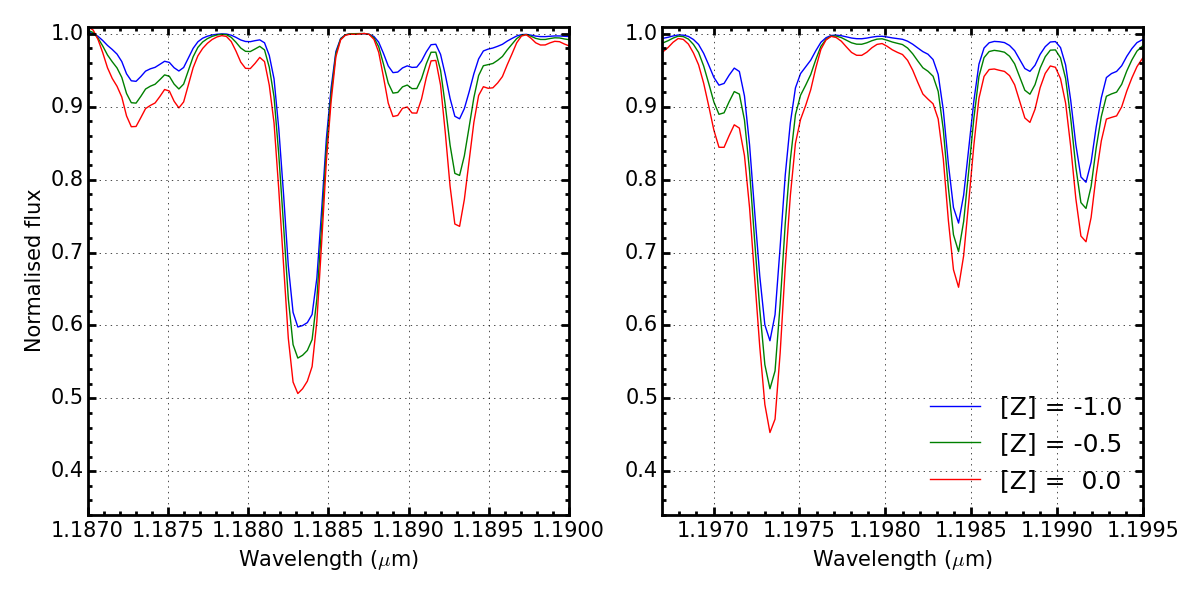
\includegraphics[width=0.65\textwidth]{JAnal/varyZv2}
\caption{
Three models where only the metallicitiy is varied.
Five diagnostic lines are shown in two panels.
Left: Fe\,I $\lambda$1.188285 and Ti\,I $\lambda$ 1.189289.
Right: Fe\,I $\lambda$ and Si\,I $\lambda\lambda$ 1.198419, 1.199157.\label{fig:mod-z}
         }
\end{figure}

\begin{figure}
 \centering
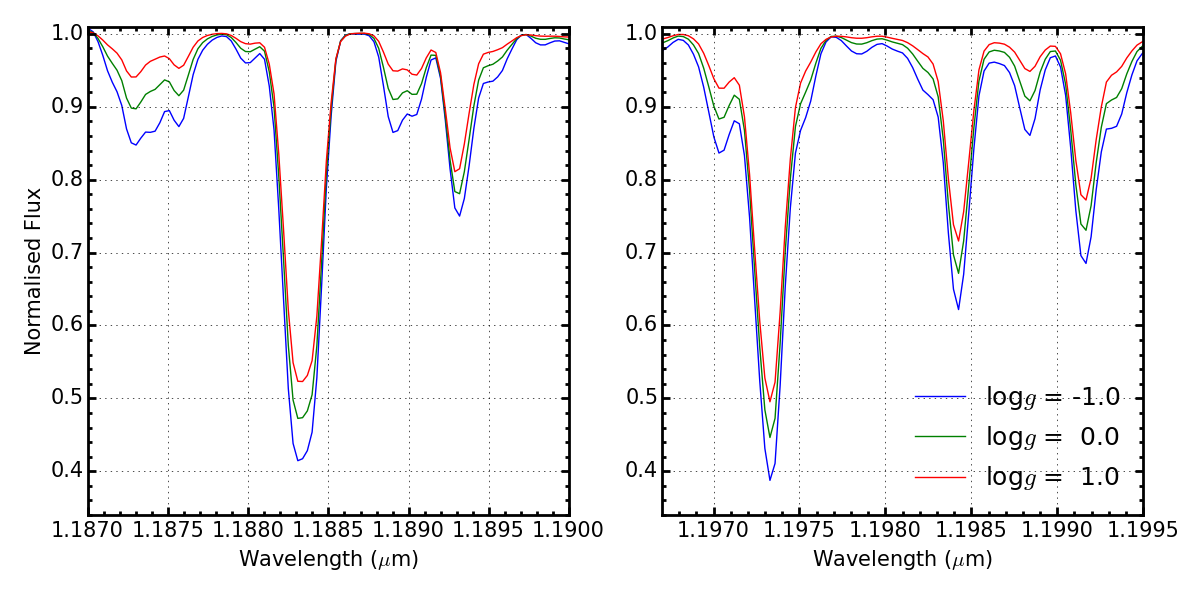
\includegraphics[width=0.65\textwidth]{JAnal/varygv2}
\caption{
As in Figure~\ref{fig:mod-z} where however surface gravity is varied.\label{fig:mod-g}
         }
\end{figure}

\begin{figure}
 \centering
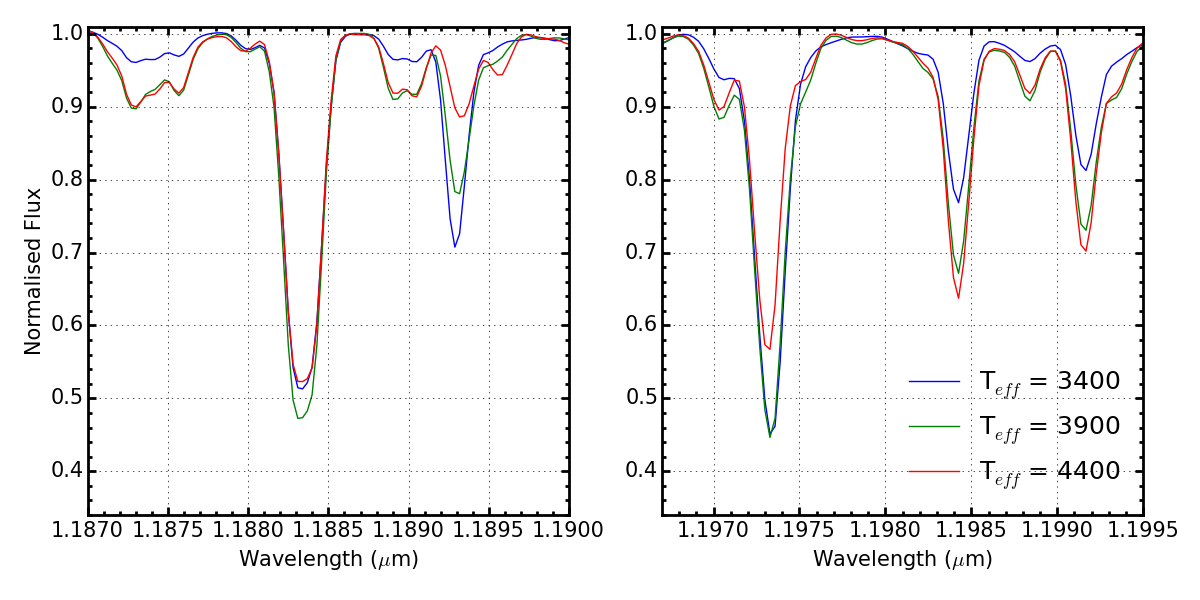
\includegraphics[width=0.65\textwidth]{JAnal/varyTv2}
\caption{
As in Figure~\ref{fig:mod-z} where however effective temperature is varied.\label{fig:mod-t}
         }
\end{figure}

\begin{figure}
 \centering
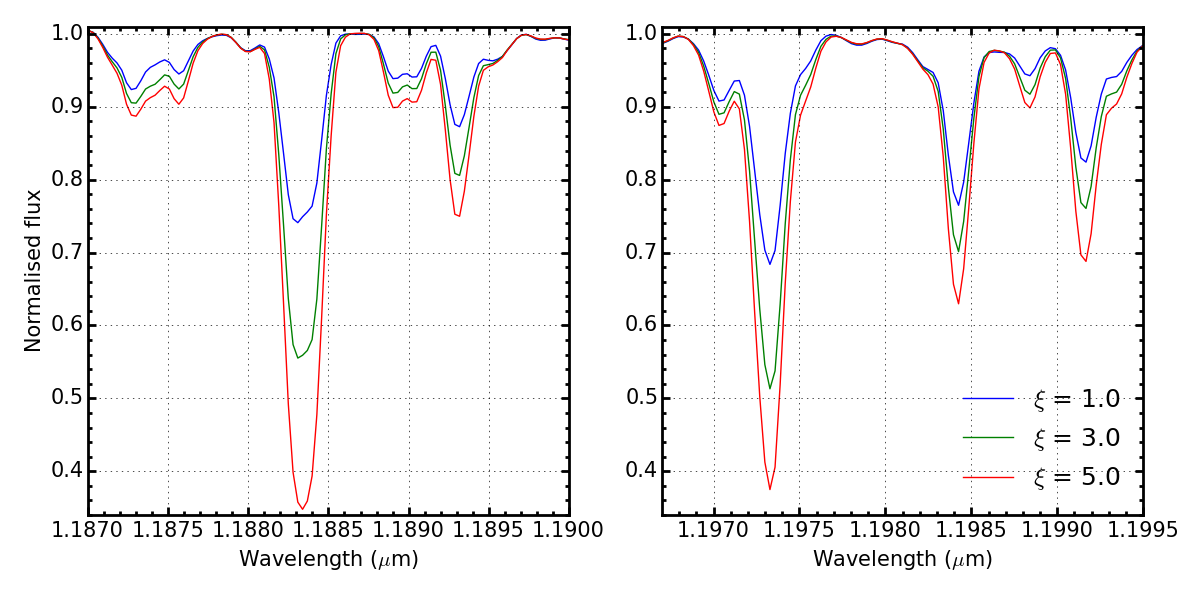
\includegraphics[width=0.65\textwidth]{JAnal/varymicrov2}
\caption{
As in Figure~\ref{fig:mod-z} where however microturblence is varied.\label{fig:mod-micro}
         }
\end{figure}

The current model grid is sufficient to explore the parameters for a typical RSG.
However, when using this technique at larger distances,
many different metallicity environments are encountered (e.g. the low metallicity environment ofI\,Zw\,18 with $Z=(1/32)Z_{\odot}$~\citep{1998ApJ...508..248V}).
In order to study these extremely low-metallicity systems,
the metallicity parameter space would need to be extended.
The $\alpha$-to-iron ratio of these stars is taken to be that of the solar value and is not left as a free parameter in the models.
This is applicable as young stars are known to have solar-like $\alpha$-to-iron ratios in different metallicity galaxies
~\citep[see tables 3 and 4 in][and references therein]{2015ApJ...806...21D}.

% \begin{itemize}
%     \item How are the grids generated?
%     \item What are the non-LTE corrections?
%     \item What do the current grids look like?
%     \item How could they be improved?
% \end{itemize}
% section model_grid (end)
\section{Continuum Fitting} % (fold)
\label{sub:continuum_fitting}

Accurately matching the continuum levels in the observed
spectrum provides a base with which to anchor the diagnostic lines of the models.
An incorrectly placed continuum level would bias the analysis and result in the
strength of the diagnostic lines being over or under estimated producing inaccurate stellar parameters.

% The continuum fitting procedure is important because determining the base of the
% diagnostic lines defines their overall strength which is used to distinguish
% between models.
There are many factors that effect the level of the continuum and continuum placement,
including the resolution of the observations as well as the stellar parameters themselves.
Therefore it is vital that when attempting to derive stellar parameters,
in crowded regions such as this, the continuum placement is performed
consistently and accurately.
Intrinsically, when studying RSGs at medium resolution - owing  to their cool atmospheres -
there are many instances of blended spectral features.
At this resolution the density of blended spectral features creates a pseudo-continuum which, in practice,
is never at the ture continnum level.
Figure~\ref{fig:mod-res} illustrates the varying continuum levels for models where the resolution is varied and
Figure~\ref{fig:mod-zcont} shows this affect when varying only the metallicity.
It can also be seen in figures~\ref{fig:mod-z}---\ref{fig:mod-micro} that each of the parameters affects the continuum in a subtly different manner.

\begin{figure}
 \centering
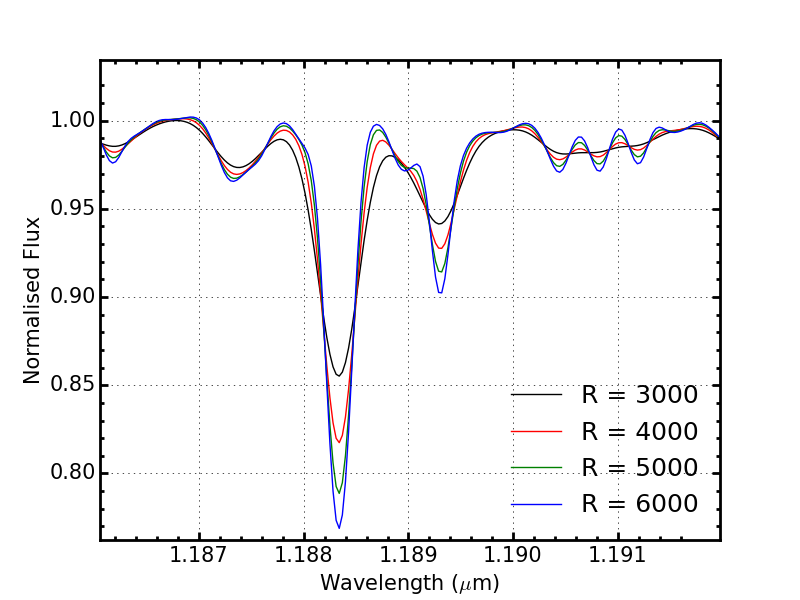
\includegraphics[width=0.65\textwidth]{JAnal/Resolution}
\caption{
One model degraded to four different resolution values.
This figure demonstrates the how the continuum level changes depending upon
the resolution of the spectrum.
We see at around 1.191$\mu$m at $R=3000$ the continuum level is perturbed by blended lines.\label{fig:mod-res}
         }
\end{figure}

\begin{figure}
 \centering
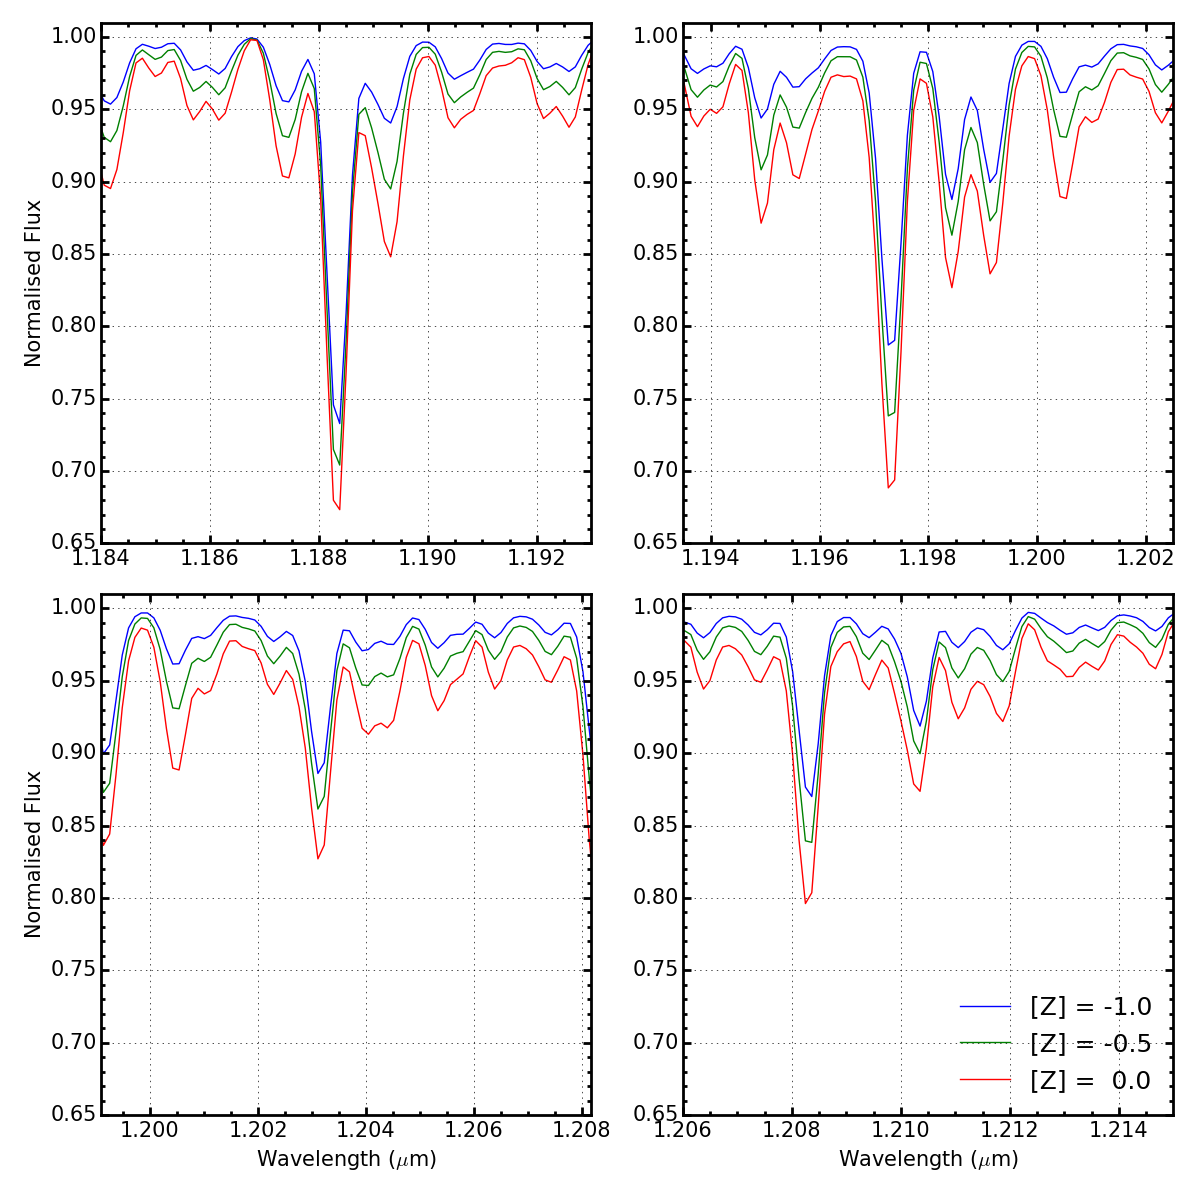
\includegraphics[width=0.65\textwidth]{JAnal/varyZ}
\caption{
Three models where only the metallicitiy is varied.
Each panel shows one or more diagnostic line.
Metallicity of the model intrinsically affects the continuum level of the spectrum,
such that at higher metallicities, there is greater departure from the true continuum level, which in the case of the models is 1.00.\label{fig:mod-zcont}
         }
\end{figure}


Given that it is impossible to know the true continuum level from any given observation,
the scaling applied must be consistent between the models and observations.
Scaling is required not only to match the levels of the continuum placement, but also to match the line strengths between the models and observations.
Providing the treatment of the models and observations are consistent, the fact that the true continuum is never attained is not significant
\citep{2014ApJ...788...58G}.
For the process of continuum matching to work effectively,
the observed and model spectra should be at the same resolution,
have a consistent wavelength calibration
and have identical spectral sampling.

In order to account for differences in the spectral sampling of the observed and model spectra,
each model spectrum is resampled onto the wavelength scale of the observations by means of a spline interpolation routine.
The model spectrum is then degraded to the resolution of the observations by a
convolution with a Gaussian filter where the width of the Gaussian is defined by the observed resolution ($FWHM~=~\sqrt{(\lambda/R)^{2} -(\lambda/R_{mod})^{2}}$ where $R$ is the resolution of the observed spectrum).
The resolution of the KMOS observations is estimated using the KMOS/esorex pipeline from arc lamp exposures at the appropriate rotator angle for the observations.
This is measured for each spectrograph and is assumed to be constant (to within $\pm 100$) across individual IFU's as well as across the detector.

% This is accounted for by degrading the sampling of the models to that of the observations by means of a linear interpolation.
% The sampling of the models are degraded to that of the observations by means of a cublic-spline interpolation.
To ensure the spectra are on the same wavelength scale, the observed specturm is cross-correlated with the model spectrum;
a shift is then applied to the observed spectrum in order to minimise the cross-correlation matrix.
This procedure is repeated until the shift between the observed and model spectra is less than $0.1\,pix$.
Over this small wavelength range, one would not expect significant variations in the spectral resolution of the observations to perturb the cross-correlation.

Once the spectra have been correctly matched they are now suitable to be compared over the wavelength range $1.165-1.215\mu$m.
To estimate the amount of scaling required first I define the continuum width ($cw$) as:

\begin{equation}
    cw~=~\frac{\lambda}{R}, %\times S,
\end{equation}
\noindent where $R$ is the resolution of the spectrum and
$\lambda$ is the wavelength at which the width is taken
(in principle this wavelength varies across the spectrum, however, given our spectral window is sufficiently small, I assume $\lambda~=~1.20\mu$m).
% and $S$ is a scale factor which takes the range $0.5 < S < 1.0$.
The continuum width is essentially the resolution element of the spectrum at a wavelength of
$\lambda~=~1.20\mu$m and defines the width in which we expect to find a combination of pixels from a spectral feature and the continuum.

% multiplied by the scale factor $S$.
% In Gazak et al. (2015) this scale factor is fixed at 0.5.
% The scale factor is introduced because ... ?

The model spectrum is divided into wavelength slices each of width $cw\mu$m and the maximum of each slice is taken.
Using this array of maxima any major feature is systematically removed by rejecting data points more than 3$\sigma$ from the mean of the distribution.
Figure~\ref{fig:cw} illustrates the width of these slices and how this technique  removes prominent spectral features.
In this figure blue points represent the boundaries between the slices of width $cw\mu$m and the maximum of each slice is shown in red.
 % using this technique systematically removes absorption features from the spectrum.
% Any remaining features in this maximum spectrum are removed by rejecting outliers which are more than 3$\sigma$ from the mean of the distribution.
% In figure~\ref{fig:cw} the $cw~max.$ points have been through this procedure.
% This can be seen by noting that the cores of the absorption lines no $cw max.$
% points present.

\begin{figure}
 \centering
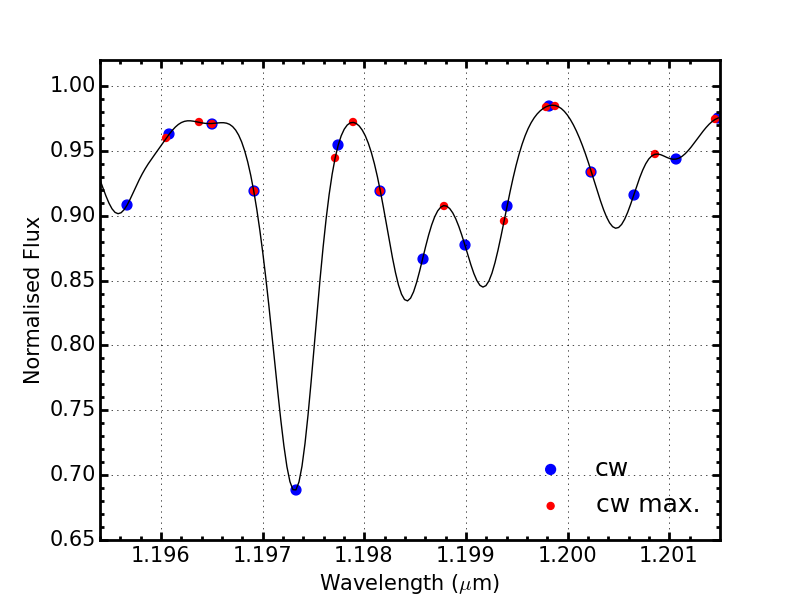
\includegraphics[width=0.65\textwidth]{JAnal/cw}
\caption[Illustration of continuum width slices and maxima]{
Illustration of the continuum width ($cw$) and slicing the model spectrum into regions of $cw\mu$m is able to remove structure in order to fit the continuum.
The solid black line shows an example of a model spectrum degraded to a resolution of 3000,
blue points show the boundaries between the slices and red points show the maximum of each slice.\label{fig:cw}
         }
\end{figure}


The remaining data points ($P_{cont}$) are used to derive an initial correction function
($cf_{1}$) by fitting a third-order polynomial to the ratio of the model to observed continuum points (red points in figure~\ref{fig:cw}), defined using the equation:
\begin{equation}
    cf_{1}~=~f(\frac{F_{mod}(P_{cont})}{F_{obs}(P_{cont})}),
\end{equation}

\noindent where $F_{mod}$ and $F_{obs}$ are the flux in the model and observed spectrum respectively.
The final correction function ($cf_{2}$), a refinement of $cf_{1}$,
is defined by removing any remaining outliers more than 3$\sigma$ from the mean of the correction function $cf_{1}$.
This method assumes that over the small wavelength range considered,
$cf_{1}$ does not vary significantly from the mean and as such, any significant deviation is considered originating from a spectral feature or noise.

The final correction function, $cf_{2}$,
is used to define the amount of scaling required for the model.
Figure~\ref{fig:cftaction} shows how the continuum fitting process works using a model spectrum as the observed spectrum (black) and a second model spectrum
(blue dashed) which is scaled to match the continuum level of the observed
(red dot-dashed).
It can be seen that the continuum placement of the example observed spectrum and that of the scaled model spectrum is well matched, even though the line strengths don't match well.

\begin{figure}
 \centering
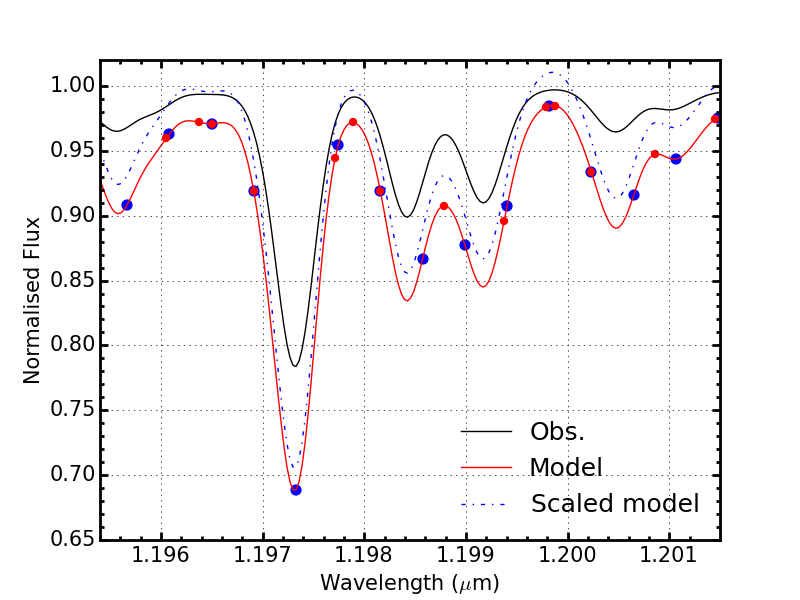
\includegraphics[width=0.65\textwidth]{JAnal/cftaction}
\caption[Example of continuum fitting]{
An example of how the continuum fitting procedure works using a model spectrum as
an example observed spectrum (black solid line)
and a separate model spectrum to match the level of the continuum.
The dashed blue spectrum denotes the model spectrum before any scaling has taken place.
The dot-dashed red spectrum denotes the model spectrum after the continuum fitting scaling has been applied.
The red and blue points the edges of the slices made and maxima of these regions respectively.
For these models, the true continuum level is at 1.00.\label{fig:cftaction}
         }
\end{figure}


% The green dashed line shows a third order polynomial fit to the ratio of the model spectrum to a simulated observed spectrum at only the red points ($~=~\frac{F_{mod}(cf_{1})}{F_{obs}(cf_{1})}$).

Alternative methods of continuum fitting are discussed in~\cite{2010MNRAS.407.1203D} and~\cite{2011A&A...527A..50E}.
These methods select pseduo-continuum pixels in the models based on ranking the model pixels and selecting a percentage of the pixels with the largest flux.
Providing the pixels from the model are selected in this manner and not those in the observations, this is a reliable method with which to derive the continuum level as demonstrated by~\cite{2015ApJ...806...21D}.
% \textbf{What advantage (if any) does the method applied here have over the one used in Davies et al. (2015 in prep.)?}

% section continuum_fitting (end)
\section{Best Fit Parameters} % (fold)
\label{sub:best_fit_parameters}

Best fit parameters are calculated using a chi-squared minimisation approach.
Each model is compared to the observed spectrum
and the chi-squared statistic is calculated using the equation,

\begin{equation}
    \chi^{2}~=~\frac{1}{N_{pix}}\sum\limits_{i}{\frac{(O_{i} - M_{i})^{2}}{\sigma^{2}}},
\end{equation}

where $N_{pix}$ is the number of pixels used and
$\sigma$ is determined by the S/N of the spectrum.
This statistic is calculated over each of the diagnostic lines and here $N_{pix}$ is the total number of pixels used to perform this calculation.
Table~\ref{tb:lines} details the diagnostic lines used in this analysis.
The amount of continuum included to compute the $\chi^{2}$-statistic is important to consider.
If this wavelength range is too small, the wings of the lines will be neglected,
which would discard vital information used to constrain the model parameters.
However, if too much of the pseudo-continuum is included, the parameters could be biased by noise features in the observations or by inaccuracies within the models.
For example,
~\cite{2014PhDT.........G} identify several spectral features present in the observed spectra which are missing in the model spectra.
The regions which are used in the calculation of the $\chi^{2}$-statistic are highlighted red in
figure~\ref{fig:lines}.
There are multiple cases where the diagnostic lines are sufficiently close together that, at R$\sim$3000,
the lines are not clearly separated.
In these instances, the most appropriate course of action is to define a region which encompasses all of the spectral features in question,
% the region where the $\chi^{2}$ is computed over all of the lines in question and to deal with the region as a whole,
as illustrated in Figure~\ref{fig:lines}.
This ensures that an individual pixel is not counted multiple times and provides a more applicable edge for which to compute the $\chi^{2}$-statistic.

\begin{figure}
 \centering
 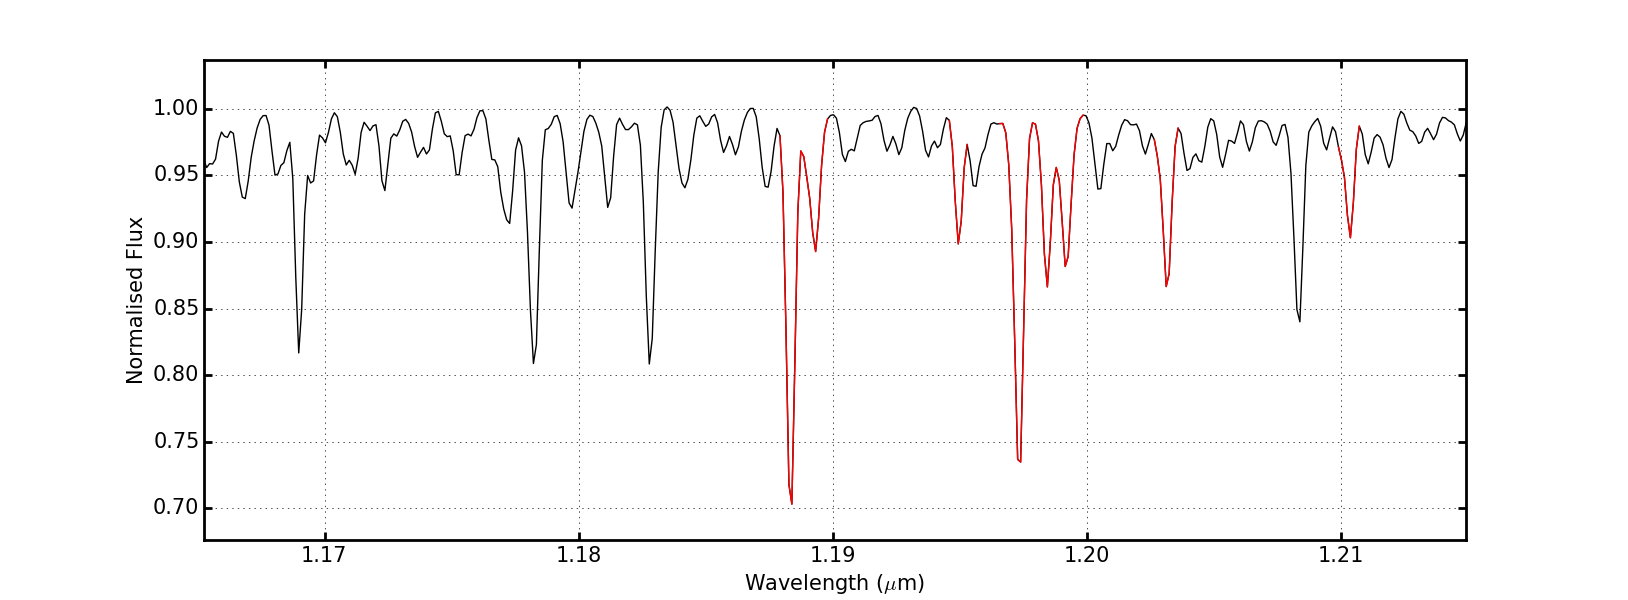
\includegraphics[width=0.65\textwidth]{JAnal/Diag-lines}
 \caption[Diagnostic lines]{
An example of a model spectrum, degraded and resampled to that of a typical observed spectrum (in this case NGC6822-RSG01), where the regions used to compute the $\chi^{2}$ calculation is highlighted in red.\label{fig:lines}
         }
\end{figure}

\begin{table}
\caption[Diagnostic lines]{Diagnostic lines\label{tb:lines}}
\scriptsize
\begin{center}
\begin{tabular}{cc}
 \hline
 \hline
Species & Line Centre \\
 \hline
Fe\,I & 1.188285 \\
Fe\,I & 1.197305 \\
Si\,I & 1.198419 \\
Si\,I & 1.199157 \\
Si\,I & 1.203151 \\
Si\,I & 1.210353 \\
Ti\,I & 1.189289 \\
Ti\,I & 1.194954 \\
Mg\,I & \\
Mg\,I & \\
 \hline
\end{tabular}
\end{center}
\end{table}

Each best fit parameter is estimated based on a weighted average,
where the weights are determined by the $\chi^{2}$ value of the model:

\begin{equation}
    w~=~exp(-\chi^{2}/2).
\end{equation}

The average is performed using the 100 models with the lowest $\chi^{2}$ value.
\begin{itemize}
    \item Why is 100 chosen?
    \item Doesn't this bias models at the edge of the grid? (e.g. figure~\ref{fig:test2})
    \item I need more on this in general!
\end{itemize}

Errors on the parameters are determined by defining
$\Delta\chi^{2}~=~\chi^{2}_{min} + 3$.
The standard deviation of the models parameters for all models which have a
$\chi^{2}$ value within this range define the errors.
For a purely Gaussin distribution the 1$\sigma$ deviation is $\Delta\chi^{2}~=~2.3$.
However, assuming one of the diagnostic lines is only fit to within 2$\sigma$ while the rest being fit to within 1$\sigma$, we obtain $(n_{l}~-~1)~\times~1^{2}~+~1~\times~2^{2}~=~n_{l}~+~3$
where $n_{l}$ is the number of lines used.

As mentioned previouslly (in~\ref{sub:model_grid}) and as demonstrated in
~\cite{2015ApJ...806...21D} there exists a degeneracy between the effect of decreasing the metallicity and increasing the surface gravity of the models.
To help break this degeneracy, I implement an additional gravity restraint.
This works by calcualting the luminosity of the observed star using near-IR photometry and the bolometric correction given in~\cite{Davies13b}.
Having calculated the luminosity, the relationship,
\begin{equation}
    \frac{g}{T^{4}_{\rm eff}}~\propto~\frac{M}{L},
\end{equation}
can be used to restrict the $log\,g$-T$_{\rm eff}$
parameter space using sensible limits for the mass of a RSG
($8~\leq~M/M_{\odot}~\leq~40$).
Where $M$ is the mass of the star,
$T_{\rm eff}$ is the effective temperature and $g$ is the surface gravity of the star.
These regions of parameter space are rejected from the analysis as unphyiscal.

To test the accuracy of the analysis routine, I begin with the most simple test I can imagine:
do I recover the parameters when using a model spectrum as input?
In every test performed in this fashion the model parameters are recovered within 1$\sigma$ across the full model grid.
To increase complexity, a small amount of noise is added to this model spectrum prior to the analysis.
Again, with all models tested (which span the full grid of model parameters) the input stellar parameters are derived to within the 1$\sigma$ errors.

The second test performed, which is a small step up in complexity, is to use a model spectrum as input, degraded to the resolution and sampling of a typical observation (in this case I use $R~=~3000$ with a sampling equal to that of the KMOS YJ grating at its natural sampling).
In addition, Gaussian noise is added to the input spectrum with the S/N~=~100
(characteristic of the poorest S/N typically observed).
The results of this test are illustrated in figure~\ref{fig:test2}.
From this figure it can be seen again that typically we see excellent agreement between the input parameters and the output parameters.
Note, all of these tests assume that the luminosity of the model is known
(idential to the assumption made when using this analysis on real data).

\begin{figure}
 \centering
 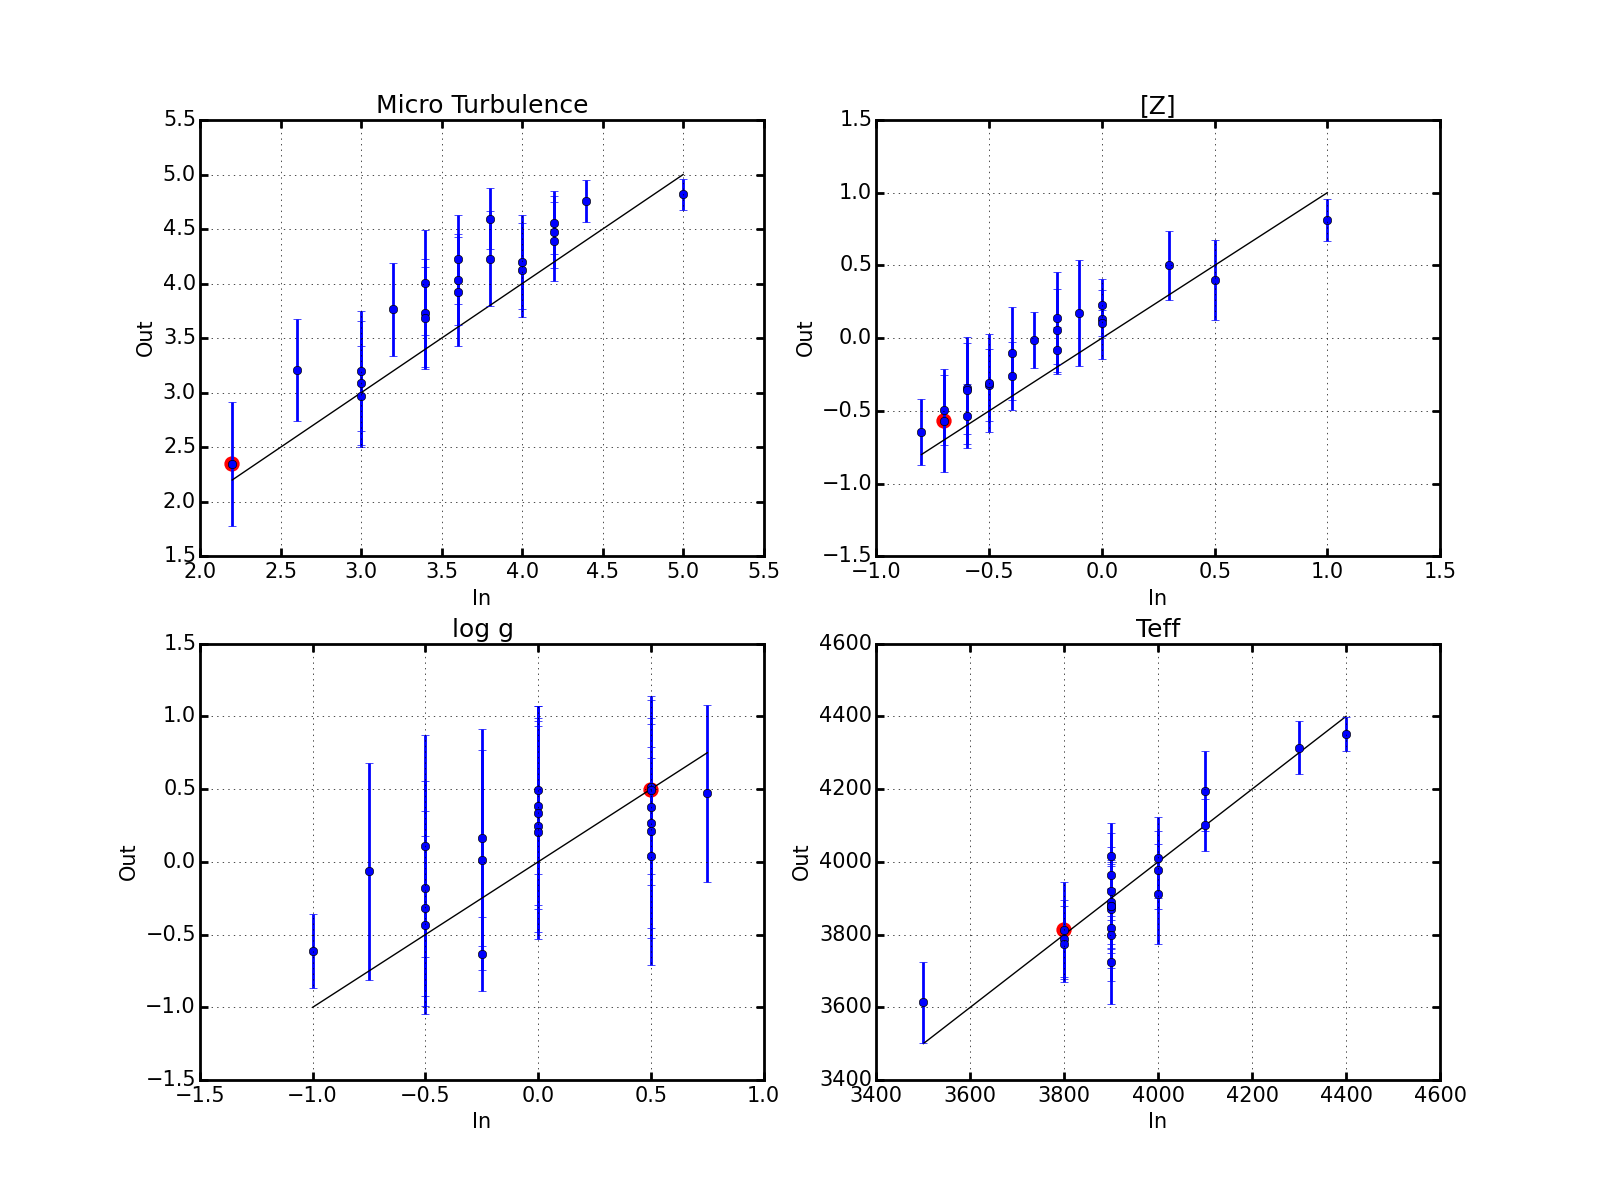
\includegraphics[width=0.65\textwidth]{JAnal/lineonly-test2v22}
 \caption[Test ]{
Results of the analysis routine using 21 fake RSG spectra as input.
The spectra span a wide range of stellar parameters and are degraded to $R~=~3000$ and resampled onto a typical sampling for the real data with random Gaussian noise added of S/N~=~100.
\label{fig:test2}
         }
\end{figure}

\section{Comparisons With Previous Implementations} % (fold)
\label{sub:compare}
To increase confidence in the accuracy and reliability of this implementation of the $J$-band synthetic spectral fitting methods,
where applicable, these routines have been compared to the results based on previous implementations of this analysis.

To date, there are currently two other published implementations using medium resolution $J$-band spectra of RSGs to derive stellar parameters,
that of~\cite[][DFK10]{2010MNRAS.407.1203D} and that of
\cite[][G14]{2014PhDT.........G}.
Both of these implementations are subtly different and use different assumptions to derive the stellar parameters.
They are both broadly based on the same techniques used in this analysis,
however, the main differences between the two methods are that DFK10 uses just the line strengths of the diagnostic lines to calculate the $\chi^{2}$ statistic,
while G14 uses the entire $1.165-1.215\,\mu$m region (with some exceptions).

In the current implementation, the diagnostic lines themselves are used to calculate the $\chi^{2}$ statistic.
This is preferred to the two aforementioned techniques for the following reasons:

1. The models used in the analysis are not perfect representations of RSG spectra.
The line list which builds these spectra are known to be incomplete and the effect of including these wavelength regions within the $\chi^{2}$ calculation could be to perturb the fit. G14 is very careful to exclude all known instances of missed lines within the models, however, this can not be assumed to be a complete consensus of missed lines.

2. Using the full line profile of the diagnostic lines provides information on the shape of the lines which using the line strength does not.

\subsection{DFK10} % (fold)
\label{sub:dfk10}
To date there have been several published articles using the DFK10 implementation
~\citep{2010MNRAS.407.1203D,2015ApJ...803...14P,2015ApJ...806...21D}.
The original implemetation was updated and tested rigourously on VLT-XSHOOTER spectra of RSGs in the Magellanic clouds in
~\cite{2015ApJ...806...21D} and in~\cite{2015ApJ...803...14P} this was applied to KMOS spectra in NGC\,6822.
In this section we compare the analysis routine detailed above with that of DFK10 on the set of 10 RSG KMOS spectra in NGC\,6822.
Figure~\ref{fig:n6822DFK} shows the comparison of the output parmaters of the stars in this sample for the two analysis routines.
This figure shows that the agreement between the two routines is acceptable for all stellar parameters.
The mean of each of the parmeters is calculated in Table~\ref{tb:DFK10} and is shown to agree within the errors.

\begin{figure}
 \centering
 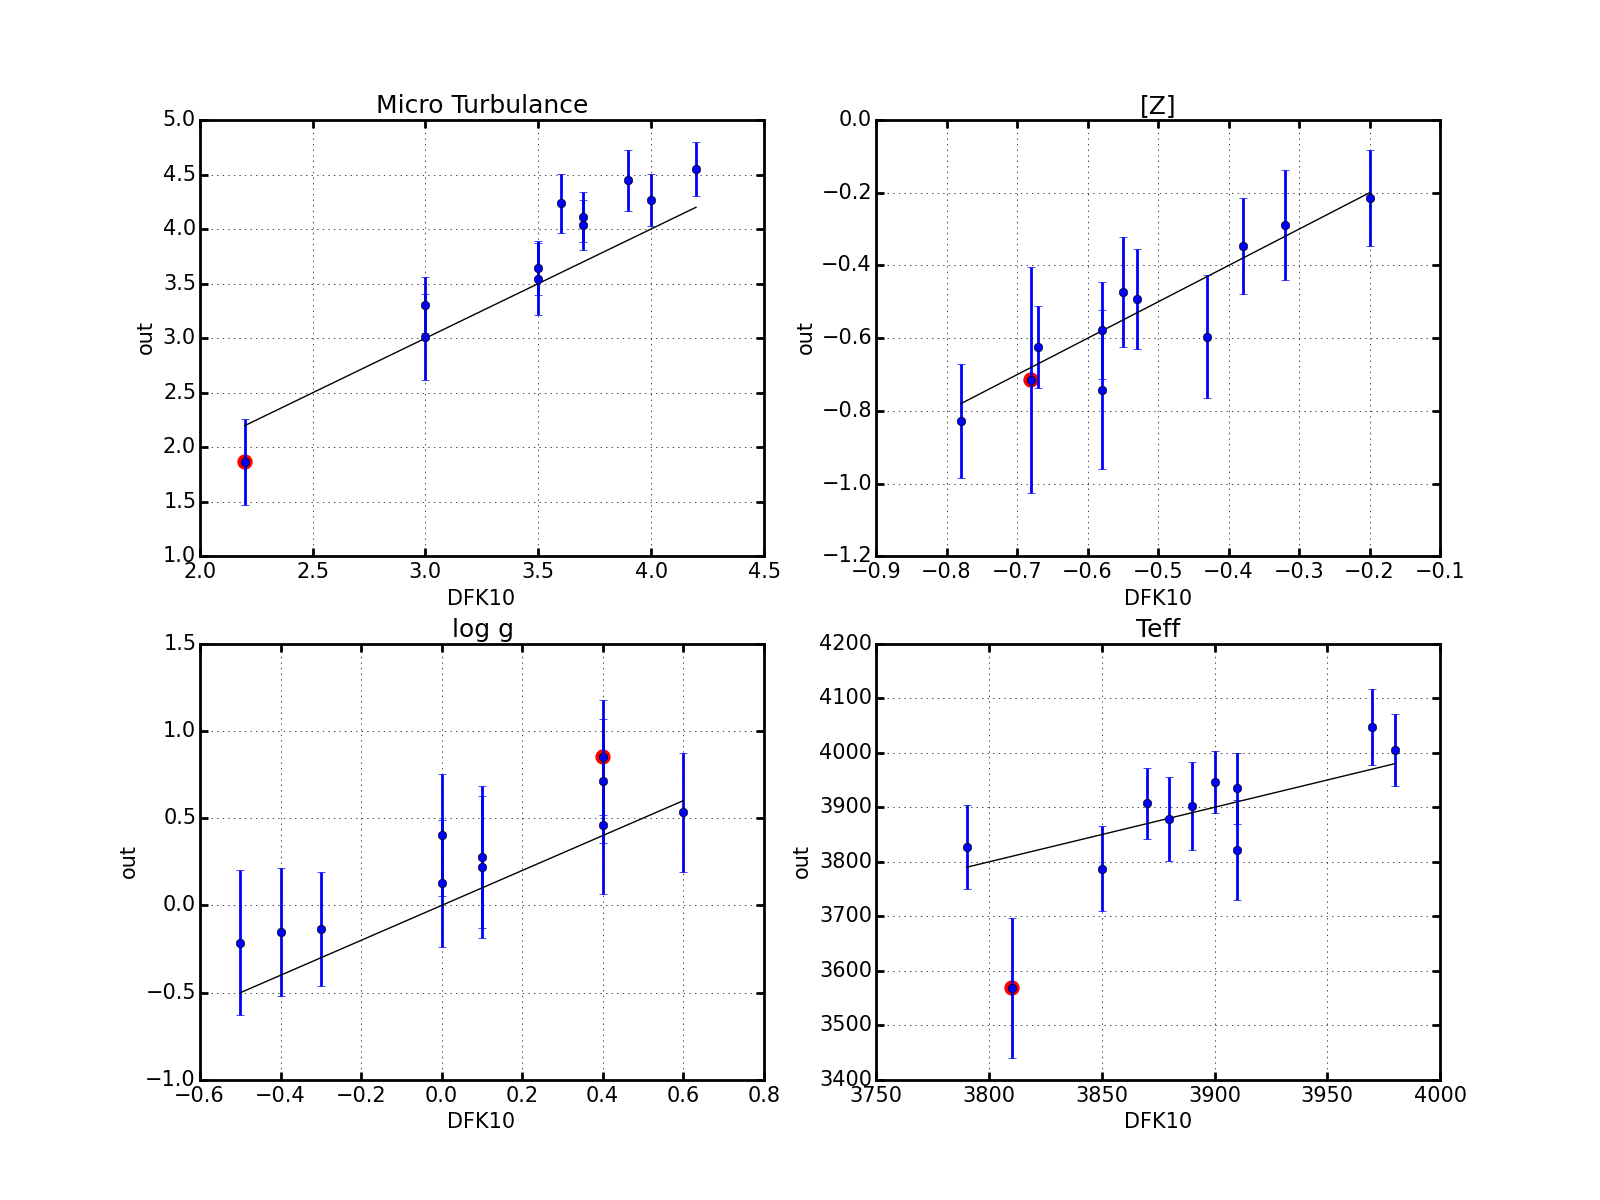
\includegraphics[width=0.65\textwidth]{JAnal/compare-DFK10}
 \caption[NGC\,6822 DFK10]{
A comparison between the parameters derived for 11 RSGs in NGC\,6822.
DFK10 results are those published in~\cite{2015ApJ...803...14P}.
\textbf{Note: I haven't commented on the offset between the parameters as I'm assuming I will be able to crack this soon!}\label{fig:n6822DFK}
         }
\end{figure}

\begin{table}
\caption[Parameter comparisons DFK10]{Average parameters for 10 RSGs in NGC\,6822 using the DFK10 implementation and the implemetation discribed here\label{tb:DFK10}}
\scriptsize
\begin{center}
\begin{tabular}{ccc}
 \hline
 \hline
Parameter & DFK10 Average & Patrick Average \\
 \hline
[Z]       & $-0.52~\pm~0.16$ &  \\
T$_{\rm eff}$ & $3887~\pm~55$ &  \\
$log\,g$  & $0.1~\pm~0.3$ &  \\
$\xi$     & $3.9~\pm~0.5$ &  \\
 \hline
\end{tabular}
\end{center}
\end{table}
% section dfk10 (end)

\section{G14} % (fold)
\label{sub:g14}
The second implementation of the $J$-band analysis technique using $J$-band spectra of RSGs was that presented and rigorously tested in~\cite{2014PhDT.........G}.
This implementation was set up to be complementary to that of DFK10 and was tested on high resolution spectra of RSGs in the Perseus OB-1 cluster.
In addition to this, this analysis was applied to KMOS spectra of 27 RSGs of NGC\,300
\citep{2015ApJ...805..182G}.

Stellar parameters have been for all spectra in NGC\,300 using the presented analysis.
In figure~\ref{fig:n300G14} I compare the results derived using the analysis presented here with those published in~\citep{2015ApJ...805..182G}.
Table~\ref{tb:G14} shows a comparison between the the mean and standard deviation of the four parameters.
The metallicity gradient is also derived for these observations and is found to compare ...

As part of the analysis G14 also fit for the resolution of the observations as a free parameter.
The resolution for each spectrum is compared to that of the values quoted in the KMOS arc-lamp calibrations.
\textbf{I'm expecting to see that these numbers are very similar}


\begin{figure}
 \centering
 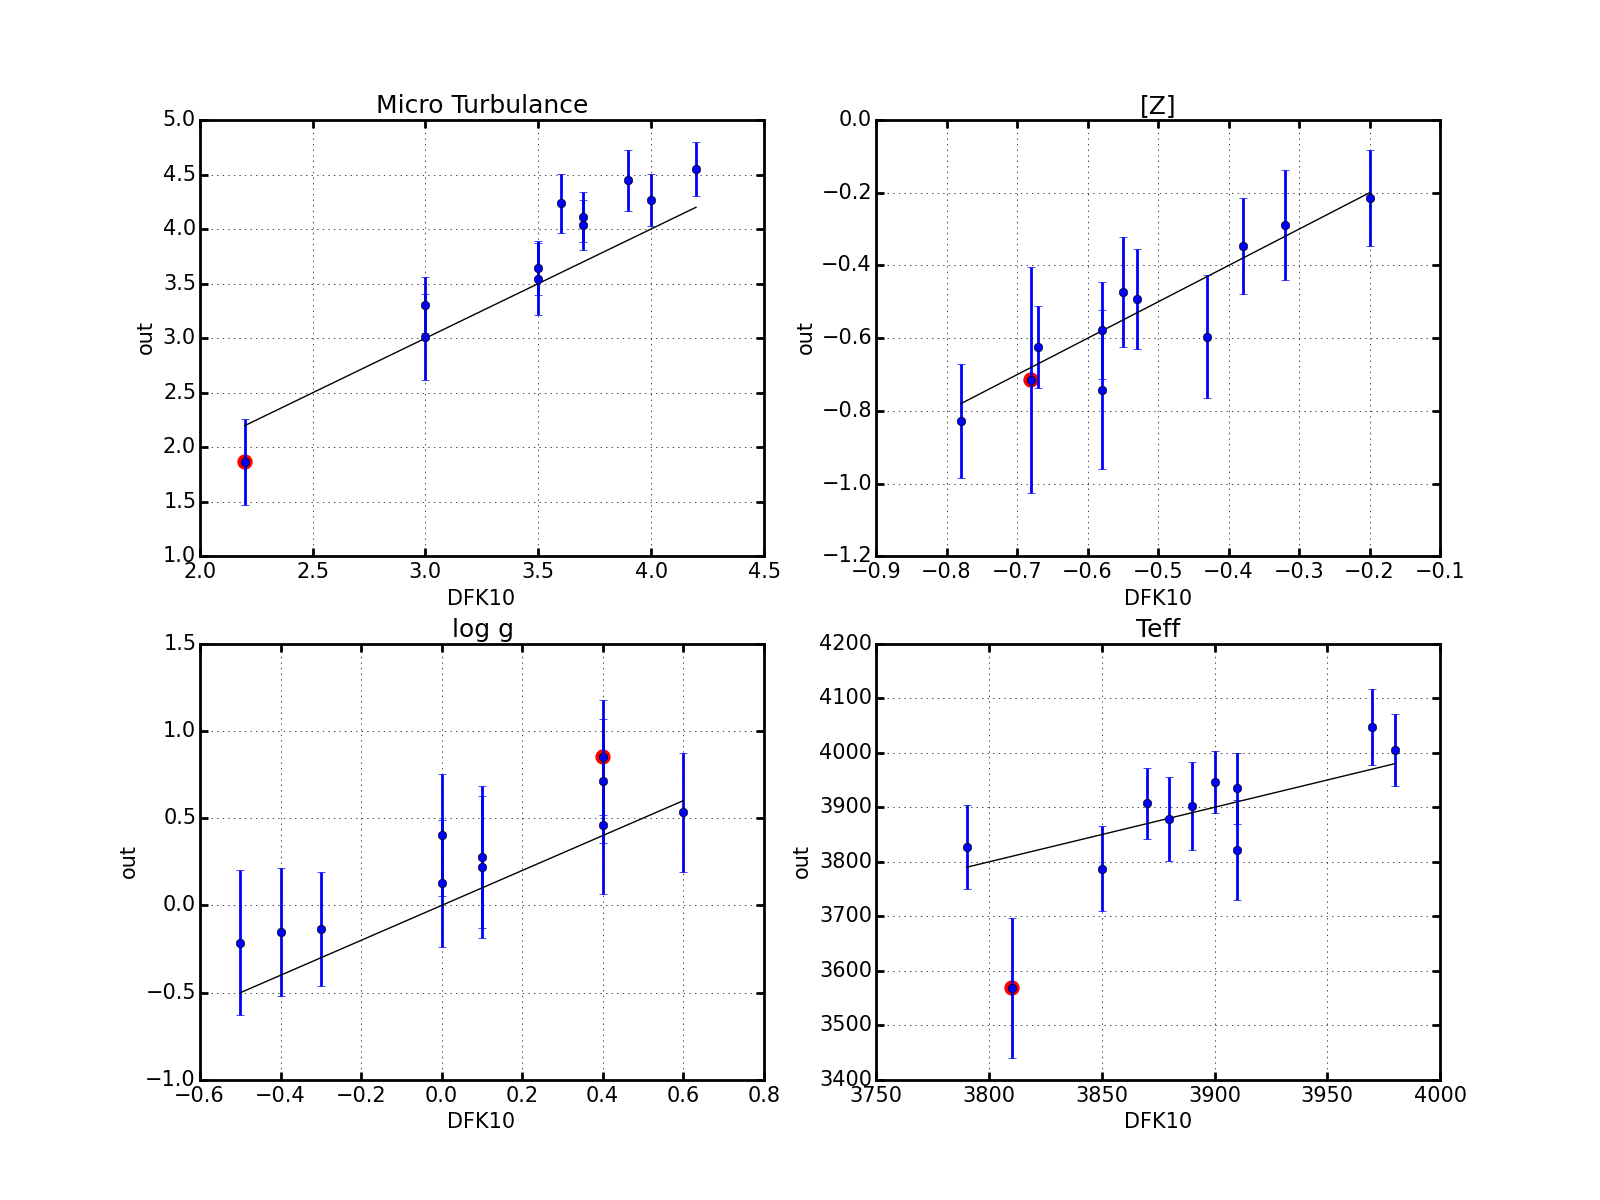
\includegraphics[width=0.65\textwidth]{JAnal/compare-DFK10}
 \caption[NGC\,300 G14]{
A comparison between the parameters derived for 27 RSGs in NGC\,300.
DFK10 results are those published in~\cite{2015ApJ...805..182G}.
\textbf{Place holder!}\label{fig:n300G14}
         }
\end{figure}

\begin{table}
\caption[Parameter comparisons G14]{Average parameters for 27 RSGs in NGC\,300 using the G14 implementation and the implementation described here
\textbf{Place holder!}\label{tb:G14}}
\scriptsize
\begin{center}
\begin{tabular}{ccc}
 \hline
 \hline
Parameter & G14 Average & Patrick Average \\
 \hline
[Z]       & $-0.52~\pm~0.16$ &  \\
T$_{\rm eff}$ & $3887~\pm~55$ &  \\
$log\,g$  & $0.1~\pm~0.3$ &  \\
$\xi$     & $3.9~\pm~0.5$ &  \\
 \hline
\end{tabular}
\end{center}
\end{table}
% section g14 (end)
% section compare (end)

\section{Conclusions} % (fold)
\label{sub:conclusions}
In this chapter I present an analysis to derive stellar parameters from RSGs using medium resolution $J$-band spectroscopy.
I detail the important aspects of this analysis including a recipe for fitting the continuum of an observed spectrum.
I describe in detail the process by which the best fit parameters and their associated errors are estimated.
I then go on to compare the results of this analysis with that of all known implementations of this analysis method and (hopefully) show that results derived between the implementations are consistent.

% subsection conclusions (end)
